\documentclass[,a4paper,12pt,french]{article}

\usepackage[TD]{../../Style}

\renewcommand\tabularxcolumn[1]{m{#1}}

\setlist[itemize]{align=parleft,left=5pt..15pt}
\setlist[enumerate]{align=parleft,left=5pt..20pt}

\geometry{centering,vcentering,left=13mm, right=13mm, top=10mm, bottom=10mm, marginparwidth=15mm}

\pagestyle{empty}

\renewcommand{\baselinestretch}{1.1}

% Début du document
%%%%%%%%%%%%%%%%%%%
\begin{document}

\titre{Exercices - Proportions, évolutions}

\begin{exercice}
En septembre 2000, la superficie minimum de la banquise arctique était de $6,32$ millions de km$^2$. Elle n'était plus que de $4,59$ millions de km$^2$ en septembre 2018. De quel pourcentage la superficie de la banquise arctique a-t-elle diminué entre septembre 2000 et septembre 2018?
\end{exercice}

\begin{exercice}
Vrai ou faux?
\begin{enumerate}
\item Après une diminution de $12 \%$, on obtient 100. Alors la valeur initiale était 112.
\item Après une augmentation de $22 \%$, on obtient 122. Alors la valeur initiale était 100.
\end{enumerate}
\end{exercice}

\begin{exercice}
La première semaine des soldes, un magasin propose $40 \%$ de réduction sur tous les vêtements. Lors de la deuxième démarque, le magasin accorde $20 \%$ de remise supplémentaire.
\begin{enumerate}
\item Calculer le coefficient multiplicateur de ces deux évolutions.
\item En déduire le coefficient multiplicateur global, puis le taux d'évolution global des prix.
\end{enumerate}
\end{exercice}

\begin{exercice}
Le tableau ci-dessous donne le PIB du Brésil et des Etats-Unis en 2000 et en 2010 (en milliards de dollars):

\compo[0.5]
{

\begin{enumerate}
\item Déterminer la variation absolue du PIB entre 2000 et 2010 pour chacun de ces pays.
\item Déterminer leur évolution relative.
\end{enumerate}
}
{
\begin{centrer}
\begin{tabularx}{0.9\linewidth}{
|>{\centering\arraybackslash}c
|>{\centering\arraybackslash}X
|>{\centering\arraybackslash}X|} \cline{2-3} \multicolumn{1}{c|}{}
& 2000 & 2010 \\ \hline
Brésil & 655 & 2209 \\ \hline
Etats-unis & 10285 & 14964 \\ \hline
\end{tabularx}
\end{centrer}
}
\end{exercice}

\begin{exercice} \

\compo[0.5]
{
Le diagramme ci-contre indique le nombre d'utilisateurs de réseaux sociaux dans le monde en 2016, 2017 et 2018:
\noindent Calculer la variation absolue, puis relative de 2016 à 2017, puis de 2017 à 2018.
}
{
\begin{centrer}
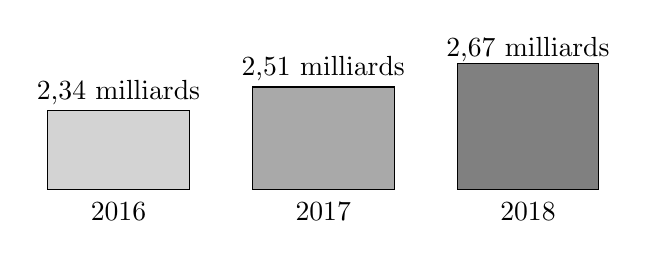
\begin{tikzpicture}
\draw[fill=LightGray] (0,0) rectangle (1.8,1) node[midway,below=5.5mm]{2016} node[midway,above=4.5mm]{2,34 milliards};
\draw[fill=DarkGray] (2.6,0) rectangle (4.4,1.3) node[midway,below=7mm]{2017} node[midway,above=6mm]{2,51 milliards};
\draw[fill=Gray] (5.2,0) rectangle (7,1.6) node[midway,below=8.5mm]{2018} node[midway,above=7mm]{2,67 milliards};
\end{tikzpicture}
\end{centrer}
}
\end{exercice}

\begin{exercice}
Une commune organise chaque année une course à pied dans les rues de son centre. En 2017, le nombre de participants a augmenté de $20 \%$ mais en 2018, il a baissé de $12 \%$. Quel est le taux d'évolution du nombre de coureurs sur ces deux années?
\end{exercice}

\begin{exercice} \

\compo[0.5]
{
Une candidate à la présidentielle 2022 a proposé de doubler le salaire des enseignants. Cette augmentation sera échelonnée sur cinq années. Voici le compte rendu qu'en a fait TF1. Que dire de ce graphique? Expliquer leur démarche.
}
{
\includegraphics[trim=35mm 45mm 15mm 3mm, clip, width=\linewidth]{"Erreur JT NB".png}
}
\end{exercice}

\newpage

\titre{Exercices - Fonctions, Généralités}

\setcounter{exercice}{0}

\begin{exercice} \

\compo[0.5]
{
Soit $f$ la fonction définie par la courbe ci-contre.
\begin{enumerate}
\item Quel est l'ensemble de définition de $f$?
\item Déterminer les images par $f$ de $-5 \ , \ 3 \ , \ -2 \ , \ 0.5$.
\item Quel est le nombre d'antécédents par $f$ de $4 \ , \ 2 \ , \ 0 \ , \ 3 , \ $?
\item Déterminer les antécédents par $f$ de $1$.
\end{enumerate}
}
{
\Centering{
\begin{tikzpicture}
\begin{axis}[
styleglobal,
width=0.9*\linewidth,
xmin=-7, xmax= 7,
ymin=-3, ymax=5,
xtick distance=1,
ytick distance=1,
minor x tick num=0,
minor y tick num=0,
tick label style = {font=\scriptsize},
]
\addplot[styleplot] plot coordinates {(-6,-2) (-5,1) (-3,2) (-1,4) (1,0) (3,-1) (4,2) (5,-1) (6,-2)} \pointsextremites;
\end{axis}
\end{tikzpicture}}
}

\end{exercice}

\begin{exercice}
Soit $f:[0;5] \rightarrow \R$ la fonction qui a $x$ associe $\frac {5x-1}{x+1}$.
\begin{enumerate}
\item Réaliser le tableau de valeurs de $f$ entre $0$ et $5$ par pas de $1$. On pourra s'aider de la calculatrice. On arrondira au dixième près.
\item A l'aide de ce tableau de valeurs, tracer dans un repère la courbe représentative de $f$ sur $[0;5]$.
\item Calculer le taux de variation de $f$ entre $2$ et $3$, puis entre $0$ et $5$.
\end{enumerate}
\end{exercice}

\begin{exercice} \
\vspace{2mm}
\compo[0.5]
{
La courbe dans le repère ci-contre représente la fonction $f$ qui à un instant $t$ exprimé en heures de l'intervalle $[0;24]$ associe la température $T$ en degrés Celsius, en un lieu.
\begin{enumerate}
\item Résoudre graphiquement l'équation $f(t)=2$. Interpréter le résultat.
\item Résoudre graphiquement l'inéquation $f(t) \geq -8$. Interpréter le résultat.
\end{enumerate}
}
{
\Centering{
\begin{tikzpicture}
\begin{axis}[
styleglobal,
hauteurproptick,
width=0.8*\linewidth,
xmin=0, xmax= 25,
ymin=-12, ymax=16,
xtick distance=2,
ytick distance=2,
minor x tick num=1,
minor y tick num=0,
ylabel={Température ($^{\circ}$C)},
xlabel={Temps (h)},
label style={font=\normalsize},
yscale=0.5,
]
\addplot[styleplot] plot coordinates {(0,10) (1,6) (2,2) (5,-4) (6,-8) (8,-10) (10,-8) (13,2) (15,8) (16,12) (18,14) (20,2) (24,-4)};
\end{axis}
\end{tikzpicture}}
}
\end{exercice}

\begin{exercice} \label{schemafonctions} \
\vspace{2mm}
\compo[0.5]
{
On se donne trois fonctions $f$, $g$ et $h$ représentées sur le repère ci-contre.
\begin{enumerate}
\item Dresser le tableau de variation de $h$.
\item Dresser le tableau de signes de $g$.
\item Dans chaque cas, résoudre:
\begin{enumerate}
\item $g(x)=h(x)$
\item $f(x) \leq h(x)$
\item $h(x) > g(x)$
\end{enumerate}
\end{enumerate}
}
{
\begin{centrer}
\begin{tikzpicture}
\begin{axis}[
styleglobal,
width=0.8*\linewidth,
xmin=-0.5, xmax= 8.5,
ymin=-2.5, ymax=3.5,
xtick distance=1,
ytick distance=1,
minor x tick num=1,
minor y tick num=1,
]
\addplot[styleplot,domain=(0:8)] plot {0.5*x-1.5)} node[pos=0.75,above] {$\mathscr C_f$};
\addplot[styleplot,color=DarkRed,densely dashed,domain=(0:8)] plot coordinates{(0,-2) (1,-1) (2,2) (3,3) (5,1) (6,0) (8,-2)} node[pos=0.6,above right] {$\mathscr C_g$};
\addplot[styleplot,densely dotted,color=DarkGreen,domain=(0:8)] plot coordinates{(0,3) (2,2) (3,0) (4,-2) (6,0) (7,2) (8,3)} node[pos=0.1,above right] {$\mathscr C_h$};
\end{axis}
\end{tikzpicture}
\end{centrer}
}
\end{exercice}

\begin{exercice}[*] \ 

\compo[0.5]
{
On se donne une fonction $f$ définie sur $[-5;4]$. On a dressé son tableau de variations et son tableau de signes ci-contre. Tracer dans un repère une courbe représentative potentielle de $f$.
}
{
\begin{centrer}
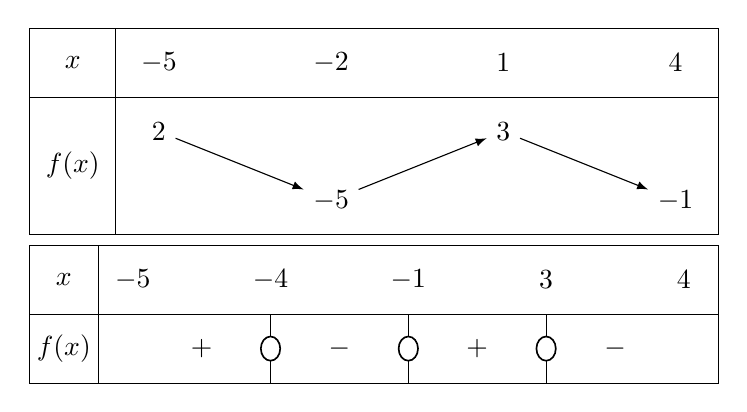
\begin{tikzpicture}[scale=0.875]
% Styles 
\tikzstyle{cadre}=[thin]
\tikzstyle{fleche}=[->,>=latex,thin]
\tikzstyle{nondefini}=[lightgray]
% Dimensions Modifiables
\def\Lrg{5/4}
\def\HtX{1}
\def\HtY{0.5}
% Dimensions Calculées
\def\lignex{-0.5*\HtX}
\def\lignef{-1.5*\HtX}
\def\separateur{-0.5*\Lrg}
% Largeur du tableau
\def\gauche{-1.5*\Lrg}
\def\droite{6.5*\Lrg}
% Hauteur du tableau
\def\haut{0.5*\HtX}
\def\bas{-1.5*\HtX-2*\HtY}
% Ligne de l'abscisse : x
\node at (-1*\Lrg,0) {$x$};
\node at (0*\Lrg,0) {$-5$};
\node at (2*\Lrg,0) {$-2$};
\node at (4*\Lrg,0) {$1$};
\node at (6*\Lrg,0) {$4$};
% Ligne de la fonction : f(x)
\node  at (-1*\Lrg,{-1*\HtX+(-1)*\HtY}) {$f(x)$};
\node (f1) at (0*\Lrg,{-1*\HtX+(0)*\HtY}) {$2$};
\node (f2) at (2*\Lrg,{-1*\HtX+(-2)*\HtY}) {$-5$};
\node (f3) at (4*\Lrg,{-1*\HtX+(0)*\HtY}) {$3$};
\node (f4) at (6*\Lrg,{-1*\HtX+(-2)*\HtY}) {$-1$};
% Flèches
\draw[fleche] (f1) -- (f2);
\draw[fleche] (f2) -- (f3);
\draw[fleche] (f3) -- (f4);
% Encadrement
\draw[cadre] (\separateur,\haut) -- (\separateur,\bas);
\draw[cadre] (\gauche,\haut) rectangle  (\droite,\bas);
\draw[cadre] (\gauche,\lignex) -- (\droite,\lignex);

\begin{scope}[shift= {(-0.38,-3.15)}]
% Styles 
\tikzstyle{cadre}=[thin]
\tikzstyle{fleche}=[->,>=latex,thin]
\tikzstyle{nondefini}=[lightgray]
% Dimensions Modifiables
\def\Lrg{1}
\def\HtX{1}
\def\HtY{0.5}
% Dimensions Calculées
\def\lignex{-0.5*\HtX}
\def\lignef{-1.5*\HtX}
\def\separateur{-0.5*\Lrg}
% Largeur du tableau
\def\gauche{-1.5*\Lrg}
\def\droite{8.5*\Lrg}
% Hauteur du tableau
\def\haut{0.5*\HtX}
\def\bas{-2.5*\HtX-2*\HtY}
% Ligne de l'abscisse : x
\node at (-1*\Lrg,0) {$x$};
\node at (0*\Lrg,0) {$-5$};
\node at (2*\Lrg,0) {$-4$};
\node at (4*\Lrg,0) {$-1$};
\node at (6*\Lrg,0) {$3$};
\node at (8*\Lrg,0) {$4$};
% Ligne de la dérivée : f'(x)
\node at (-1*\Lrg,-1*\HtX) {$f(x)$};
\node at (0*\Lrg,-1*\HtX) {$ $};
\node at (1*\Lrg,-1*\HtX) {$+$};
\draw[cadre] (2*\Lrg,-0.5*\HtX) -- (2*\Lrg,-1.5*\HtX) node[pos=0.5,line width=0.6pt,draw=black,circle,minimum size=7pt,fill=white,inner sep=2pt,yscale=1.25] {};
\node at (3*\Lrg,-1*\HtX) {$-$};
\draw[cadre] (4*\Lrg,-0.5*\HtX) -- (4*\Lrg,-1.5*\HtX) node[pos=0.5,line width=0.6pt,draw=black,circle,minimum size=7pt,fill=white,inner sep=2pt,yscale=1.25] {};
\node at (5*\Lrg,-1*\HtX) {$+$};
\draw[cadre] (6*\Lrg,-0.5*\HtX) -- (6*\Lrg,-1.5*\HtX) node[pos=0.5,line width=0.6pt,draw=black,circle,minimum size=7pt,fill=white,inner sep=2pt,yscale=1.25] {};
\node at (7*\Lrg,-1*\HtX) {$-$};
\node at (8*\Lrg,-1*\HtX) {$ $};
% Ligne de la fonction : f(x)
% Encadrement
\draw[cadre] (\separateur,\haut) -- (\separateur, \lignef);
\draw[cadre] (\gauche,\haut) rectangle  (\droite, \lignef);
\draw[cadre] (\gauche,\lignex) -- (\droite,\lignex);
\end{scope}
\end{tikzpicture}
\end{centrer}
}
\end{exercice}

\newpage

\titre{Exercices - Suites, Généralités}

\setcounter{exercice}{0}

\begin{exercice} \
\begin{enumerate}
\item Soit $u$ une suite de premier terme $u_{57}$. Déterminer l'indice du troisième et du septième terme.
\item Donner une hypothèse concernant l'indice du millième terme de cette suite.
\item Soit $v$ la suite définie sur $\N$ par $u_n=3n-2$. Déterminer $v_0, v_1, v_2, v_{10}$.
\item Soit $w$ la suite telle que $w_0=1$ et pour $n \in N, w_{n+1}=5-2w_n$. Déterminer $w_1, w_2, w_3$.
\end{enumerate}
\end{exercice}

\begin{exercice}
Représenter la suite $u$ définie sur $\N$ par $u_n=\frac {n \times \sqrt n} 3$, et établir une conjecture sur son sens de variation.
\end{exercice}

\begin{exercice} \

\begin{enumerate}
\item Recopier et compléter le schéma suivant:

\noindent 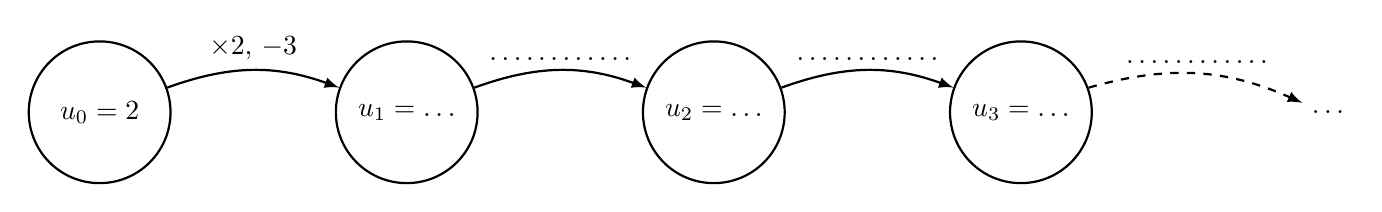
\begin{tikzpicture}[scale=1.3]
\node[draw,circle,thick, minimum size=18mm] (W0) at (-3,0) {$u_0=2$};
\node[draw,circle,thick, minimum size=18mm] (W1) at (0,0) {$u_1=\ldots$};
\node[draw,circle,thick, minimum size=18mm] (W2) at (3,0) {$u_2=\ldots$};
\node[draw,circle,thick, minimum size=18mm] (W3) at (6,0) {$u_3=\ldots$};
\node (W4) at (9,0) {$\ldots$};
\draw[->,>=latex,thick] (W0) to[bend left=20] node[midway,above]{$\times 2$, $-3$} (W1);
\draw[->,>=latex,thick] (W1) to[bend left=20] node[midway,above]{$\makebox[2cm]{\dotfill}$} (W2);
\draw[->,>=latex,thick] (W2) to[bend left=20] node[midway,above]{$\makebox[2cm]{\dotfill}$} (W3);
\draw[->,>=latex,thick,dashed] (W3) to[bend left=20] node[midway,above]{$\makebox[2cm]{\dotfill}$} (W4);
\end{tikzpicture}

\item Déterminer la relation de récurrence vérifiée par $u$.
\item Soit $w$ une suite telle que $w_0=2$ et pour $n \in \N$, $w_{n+1}=w_n \times (1-w_n)$. Calculer $w_1, \ldots, w_4$.
\item Que dire des variations de la suite? Justifier.
\end{enumerate}
\end{exercice}

\begin{exercice}
On définit la suite $u$ sur $\N$ par $u_n=3n$. On pose ensuite $v$ la suite telle que pour $n \in \N, v_n=u_{n+1}$. Déterminer $v_n$ en fonction de $n$.
\end{exercice}

\begin{exercice}
Soit $u$ la suite définie sur $\N$ par $u_n=5-2n$.
\begin{enumerate}
\item Remplacer $n$ par $n+1$ dans la formule définissant $u$. En déduire $u_{n+1}$ en fonction de $n$.
\item Calculer alors $u_{n+1}-u_n$.
\item En déduire le sens de variation de $u$.
\end{enumerate}
\end{exercice}

\begin{exercice}
On se donne la suite $v$ définie pour tout $n \in \N$ par $v_n=3-2n$.
\begin{enumerate}
\item Représenter les six premiers termes de la suite $v$ dans un repère
\item Emettre puis prouver une conjecture concernant les variations de $v$.
\end{enumerate}
\end{exercice}

\begin{exercice} \

\compo[0.35]
{
On se donne la suite $h$ représentée ci-contre.
\begin{enumerate}
\item Déterminer le premier terme de la suite, $u_4$ et $u_7$.
\item Etablie une conjecture concernant les variations de $h$.
\item Peut-on en être certain?
\end{enumerate}
}
{
\begin{centrer}
\begin{tikzpicture}
\begin{axis}[
styleglobal,
width=0.8*\linewidth,
xmin=-0.5, xmax= 8.5,
ymin=-1.5, ymax=4,
xtick distance=1,
ytick distance=1,
minor x tick num=1,
minor y tick num=1,
xlabel={$n$},
ylabel={$h_n$},
]
\addplot[draw=none,domain=(0:8),samples=9,mark=*] plot {0.3*sin(deg(x))+1.5*ln(x+0.8)};
\end{axis}
\end{tikzpicture}
\end{centrer}
}
\end{exercice}

\end{document}
